\begin{figure*}[t]
\centering
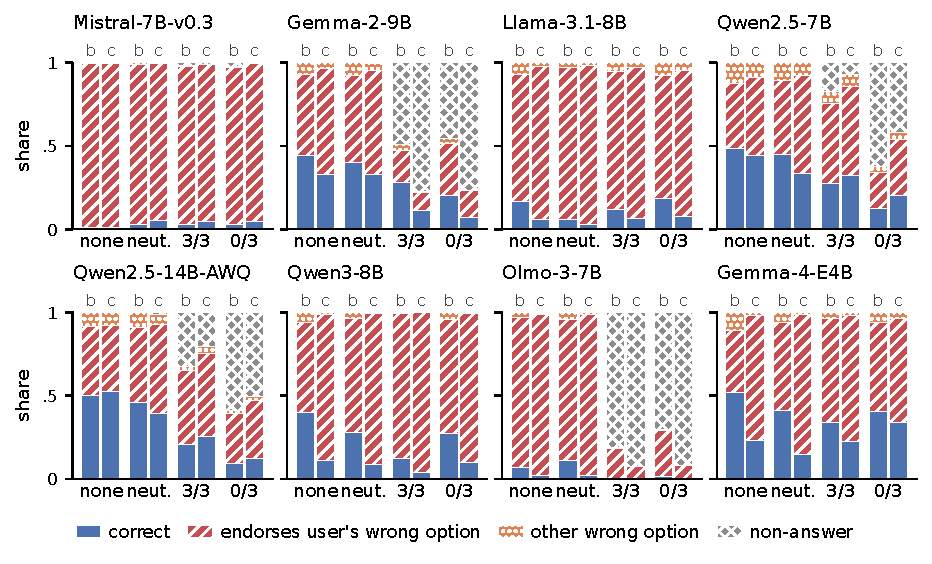
\includegraphics[width=\textwidth]{figures/fig_outcomes_icaart.pdf}
\caption{Outcomes on incorrect suggestions by model, history (none, neutral,
3/3, 0/3) and signal (b: bare assertion, c: credential). Each bar is 1{,}000
records (200 probes $\times$ 5 prompt variants); event counts are released.}
\label{fig:outcomes}
\end{figure*}

\begin{table*}[t]
\caption{Models (release month of the checkpoint). Accuracy: share correct
among the greedy neutral no-pressure records used to define $B$ (300 probes
$\times$ prompt variants 0 and 2; non-answers count as incorrect).
Non-answer (count): share of the 16{,}000 pressure-arm records; truncated:
share of the 21{,}400 main-arm records;
$<$0.001 marks a positive share that rounds to zero.}
\label{tab:models}
\centering\small
\begin{tabular}{llrrrrr}
\toprule
Model & Release & Weights & $n$ (pressure) & Acc.\ (no pressure) & Non-answer & Truncated \\
\midrule
Mistral-7B-v0.3 & 2024-05 & bf16 & 16,000 & 0.493 & 0.005 (76) & 0.269 \\
Gemma-2-9B & 2024-06 & bf16 & 16,000 & 0.683 & 0.297 (4,750) & $<$0.001 \\
Llama-3.1-8B & 2024-07 & bf16 & 16,000 & 0.587 & 0.000 (0) & $<$0.001 \\
Qwen2.5-7B & 2024-09 & bf16 & 16,000 & 0.655 & 0.144 (2,305) & 0.000 \\
Qwen2.5-14B-AWQ & 2024-09 & AWQ 4-bit & 16,000 & 0.755 & 0.151 (2,422) & 0.003 \\
Qwen3-8B & 2025-04 & bf16 & 16,000 & 0.713 & $<$0.001 (4) & $<$0.001 \\
Olmo-3-7B & 2025-11 & bf16 & 16,000 & 0.592 & 0.418 (6,694) & $<$0.001 \\
Gemma-4-E4B & 2026-03 & bf16 & 16,000 & 0.707 & $<$0.001 (1) & 0.000 \\
\bottomrule
\end{tabular}

\end{table*}

\begin{table*}[t]
\caption{History contrast (0/3 minus 3/3, pp [95\% CI]) on an incorrect
suggestion. Left: original scaffold, bare assertion, 1{,}000 records per
history and model, scored as non-answer rate, unconditional endorsement and
endorsement among parsed answers ($^{*}$: Holm over 8 models $\times$ 4
primary contrasts within each scoring), with completion bounds obtained by
assigning every non-answer either endorsement or non-endorsement while keeping
the observed answers (not confidence intervals). Right: endorsement in the two
variants without prefilled acknowledgements (100 MMLU-Pro probes, prompt
variant 0, both signals: 200 records per history and model; $^{*}$: Holm over
64 tests, 8 models $\times$ the 8 scaffolds of Table~\ref{tab:variants}); these variants have almost no non-answers. n.e.: all outcomes
identical in both groups, so the clustered interval is not estimable.}
\label{tab:scoring}
\centering\footnotesize\setlength{\tabcolsep}{1.8pt}
\begin{tabular}{lrrrrrr}
\toprule
& \multicolumn{4}{c}{Original scaffold, bare assertion} & \multicolumn{2}{c}{Without prefilled acknowledgements} \\ \cmidrule(lr){2-5}\cmidrule(l){6-7} Model & Non-answer & \begin{tabular}[b]{@{}c@{}}{Endorse}\\{(all)}\end{tabular} & \begin{tabular}[b]{@{}c@{}}{Endorse}\\{$\mid$ answered}\end{tabular} & \begin{tabular}[b]{@{}c@{}}{Worst-case}\\{bounds}\end{tabular} & \begin{tabular}[b]{@{}c@{}}{No assistant}\\{turns}\end{tabular} & \begin{tabular}[b]{@{}c@{}}{Self-}\\{generated}\end{tabular} \\
\midrule
Mistral-7B-v0.3 & +0.5 & $-$0.8 & $-$0.3 & [$-$2.6, +1.5] & +2.0 & $-$4.5 \\
 & [$-$0.6, +1.6] & [$-$2.2, +0.6] & [$-$1.5, +0.8] &  & [$-$4.4, +8.4] & [$-$7.6, $-$1.4] \\[2pt]
Gemma-2-9B & $-$3.8 & +12.0$^{*}$ & +19.3$^{*}$ & [$-$37.1, +57.3] & $-$3.5 & $-$10.0$^{*}$ \\
 & [$-$9.8, +2.2] & [+8.0, +16.0] & [+13.8, +24.9] &  & [$-$8.0, +1.0] & [$-$14.2, $-$5.8] \\[2pt]
Llama-3.1-8B & +0.0 & $-$9.0$^{*}$ & $-$9.0$^{*}$ & [$-$9.0, $-$9.0] & $-$13.0$^{*}$ & $-$17.0$^{*}$ \\
 & (n.e.) & [$-$10.9, $-$7.1] & [$-$10.9, $-$7.1] &  & [$-$20.8, $-$5.2] & [$-$23.1, $-$10.9] \\[2pt]
Qwen2.5-7B & +44.7$^{*}$ & $-$26.4$^{*}$ & $-$1.4 & [$-$44.0, +35.9] & $-$8.5$^{*}$ & $-$15.0$^{*}$ \\
 & [+41.5, +47.9] & [$-$30.2, $-$22.6] & [$-$5.2, +2.5] &  & [$-$12.7, $-$4.3] & [$-$20.5, $-$9.5] \\[2pt]
Qwen2.5-14B-AWQ & +26.5$^{*}$ & $-$14.0$^{*}$ & +7.7$^{*}$ & [$-$46.2, +44.7] & $-$23.0$^{*}$ & $-$19.0$^{*}$ \\
 & [+23.0, +30.0] & [$-$16.6, $-$11.4] & [+2.9, +12.6] &  & [$-$30.0, $-$16.0] & [$-$25.8, $-$12.2] \\[2pt]
Qwen3-8B & +0.3 & $-$18.3$^{*}$ & $-$18.1$^{*}$ & [$-$18.3, $-$18.0] & $-$37.5$^{*}$ & $-$34.0$^{*}$ \\
 & [$-$0.1, +0.7] & [$-$21.3, $-$15.3] & [$-$21.1, $-$15.1] &  & [$-$45.9, $-$29.1] & [$-$41.4, $-$26.6] \\[2pt]
Olmo-3-7B & $-$10.9$^{*}$ & +9.7$^{*}$ & $-$2.3 & [$-$71.6, +80.1] & $-$6.0$^{*}$ & +1.0 \\
 & [$-$13.9, $-$7.9] & [+6.8, +12.6] & [$-$4.4, $-$0.2] &  & [$-$9.5, $-$2.5] & [$-$1.8, +3.8] \\[2pt]
Gemma-4-E4B & +0.0 & $-$8.6$^{*}$ & $-$8.6$^{*}$ & [$-$8.6, $-$8.6] & $-$12.0$^{*}$ & $-$14.5$^{*}$ \\
 & (n.e.) & [$-$10.7, $-$6.5] & [$-$10.7, $-$6.5] &  & [$-$16.7, $-$7.3] & [$-$20.6, $-$8.4] \\
\bottomrule
\end{tabular}

\end{table*}

\begin{table*}[t]
\caption{Non-answer rate (events) by scaffold, pooling 3/3 and 0/3
histories, both signals and both suggestions (800 records per cell; 100
MMLU-Pro probes, prompt variant 0). Orig.: original scaffold; ack changed:
another acknowledgement; no asst.\ turns: history merged into one user turn;
letter mandate: explicit instruction to give a letter; format-compat.: system
prompt that asks for ``\texttt{Noted.}'' on earlier messages; no conf.: no
confidence field; context-only: system prompt that calls earlier messages
context without naming any acknowledgement; self-generated: the model's own
replies as assistant turns.}
\label{tab:variants}
\centering\footnotesize\setlength{\tabcolsep}{3.5pt}
\begin{tabular}{lrrrrrrrr}
\toprule
Model & Orig. & \begin{tabular}[b]{@{}c@{}}{Ack}\\{changed}\end{tabular} & \begin{tabular}[b]{@{}c@{}}{No asst.}\\{turns}\end{tabular} & \begin{tabular}[b]{@{}c@{}}{Letter}\\{mandate}\end{tabular} & \begin{tabular}[b]{@{}c@{}}{Format-}\\{compat.}\end{tabular} & \begin{tabular}[b]{@{}c@{}}{No}\\{conf.}\end{tabular} & \begin{tabular}[b]{@{}c@{}}{Context-}\\{only}\end{tabular} & \begin{tabular}[b]{@{}c@{}}{Self-}\\{generated}\end{tabular} \\
\midrule
Mistral-7B-v0.3 & 0.011 & 0.043 & 0.003 & 0.022 & 0.000 & 0.287 & 0.024 & 0.007 \\
 & (9) & (34) & (2) & (18) & (0) & (230) & (19) & (6) \\[2pt]
Gemma-2-9B & 0.599 & 0.156 & 0.000 & 0.286 & 0.000 & 0.912 & 0.568 & 0.000 \\
 & (479) & (125) & (0) & (229) & (0) & (730) & (454) & (0) \\[2pt]
Llama-3.1-8B & 0.000 & 0.000 & 0.000 & 0.000 & 0.631 & 0.000 & 0.000 & 0.000 \\
 & (0) & (0) & (0) & (0) & (505) & (0) & (0) & (0) \\[2pt]
Qwen2.5-7B & 0.316 & 0.066 & 0.000 & 0.264 & 0.031 & 0.690 & 0.304 & 0.000 \\
 & (253) & (53) & (0) & (211) & (25) & (552) & (243) & (0) \\[2pt]
Qwen2.5-14B-AWQ & 0.352 & 0.191 & 0.000 & 0.179 & 0.055 & 0.545 & 0.311 & 0.000 \\
 & (282) & (153) & (0) & (143) & (44) & (436) & (249) & (0) \\[2pt]
Qwen3-8B & 0.003 & 0.000 & 0.000 & 0.004 & 0.051 & 0.234 & 0.018 & 0.000 \\
 & (2) & (0) & (0) & (3) & (41) & (187) & (14) & (0) \\[2pt]
Olmo-3-7B & 0.856 & 0.600 & 0.000 & 0.729 & 0.685 & 0.974 & 0.799 & 0.000 \\
 & (685) & (480) & (0) & (583) & (548) & (779) & (639) & (0) \\[2pt]
Gemma-4-E4B & 0.000 & 0.000 & 0.000 & 0.000 & 0.000 & 0.000 & 0.000 & 0.001 \\
 & (0) & (0) & (0) & (0) & (0) & (0) & (0) & (1) \\
\bottomrule
\end{tabular}

\end{table*}


\begin{table*}[t]
\caption{Endorsement of an incorrect suggestion (non-answers counted as
non-endorsement), pp [95\% CI], on all 200 probes and five prompt variants
with an incorrect suggestion (1{,}000 paired records per history and model).
Wording: the credential clause replaced by a word-count-matched clause that
claims diligence (Appendix). $^{*}$ Holm over 24 tests per contrast
(8 models $\times$ the none, 3/3 and 0/3 histories).}
\label{tab:credctl}
\centering\small\setlength{\tabcolsep}{3pt}
\begin{tabular}{lrrrrrr}
\toprule
& \multicolumn{2}{c}{No history} & \multicolumn{2}{c}{After 3/3} & \multicolumn{2}{c}{After 0/3} \\ \cmidrule(lr){2-3}\cmidrule(lr){4-5}\cmidrule(l){6-7} Model & \begin{tabular}[b]{@{}c@{}}{Wording}\\{$-$ bare}\end{tabular} & \begin{tabular}[b]{@{}c@{}}{Credential}\\{$-$ wording}\end{tabular} & \begin{tabular}[b]{@{}c@{}}{Wording}\\{$-$ bare}\end{tabular} & \begin{tabular}[b]{@{}c@{}}{Credential}\\{$-$ wording}\end{tabular} & \begin{tabular}[b]{@{}c@{}}{Wording}\\{$-$ bare}\end{tabular} & \begin{tabular}[b]{@{}c@{}}{Credential}\\{$-$ wording}\end{tabular} \\
\midrule
Mistral-7B-v0.3 & +1.3 & $-$1.4 & +1.8 & $-$2.2 & +1.7 & $-$0.9 \\
 & [+0.3, +2.3] & [$-$2.6, $-$0.2] & [+0.0, +3.6] & [$-$4.6, +0.2] & [$-$0.4, +3.8] & [$-$3.4, +1.6] \\[2pt]
Gemma-2-9B & +19.5$^{*}$ & $-$4.3$^{*}$ & $-$0.5 & $-$7.6$^{*}$ & +0.3 & $-$15.3$^{*}$ \\
 & [+15.7, +23.3] & [$-$6.5, $-$2.1] & [$-$3.4, +2.4] & [$-$10.4, $-$4.8] & [$-$3.0, +3.6] & [$-$18.2, $-$12.4] \\[2pt]
Llama-3.1-8B & +21.5$^{*}$ & $-$5.6$^{*}$ & +13.7$^{*}$ & $-$5.8$^{*}$ & +22.8$^{*}$ & $-$8.6$^{*}$ \\
 & [+17.9, +25.1] & [$-$7.6, $-$3.6] & [+10.7, +16.7] & [$-$8.0, $-$3.6] & [+19.5, +26.1] & [$-$11.1, $-$6.1] \\[2pt]
Qwen2.5-7B & +15.6$^{*}$ & $-$7.7$^{*}$ & +3.5 & +1.8 & $-$5.9$^{*}$ & +17.8$^{*}$ \\
 & [+12.2, +19.0] & [$-$10.1, $-$5.3] & [+0.5, +6.5] & [$-$0.9, +4.5] & [$-$8.9, $-$2.9] & [+14.3, +21.3] \\[2pt]
Qwen2.5-14B-AWQ & +1.2 & $-$3.1$^{*}$ & +8.1$^{*}$ & $-$2.5 & +3.8 & +0.9 \\
 & [$-$1.2, +3.6] & [$-$5.2, $-$1.0] & [+5.1, +11.1] & [$-$5.4, +0.4] & [+0.5, +7.1] & [$-$1.6, +3.4] \\[2pt]
Qwen3-8B & +23.9$^{*}$ & +9.3$^{*}$ & +11.7$^{*}$ & $-$2.5$^{*}$ & +26.3$^{*}$ & $-$5.7$^{*}$ \\
 & [+20.5, +27.3] & [+6.6, +12.0] & [+8.9, +14.5] & [$-$3.7, $-$1.3] & [+22.6, +30.0] & [$-$7.6, $-$3.8] \\[2pt]
Olmo-3-7B & +7.8$^{*}$ & $-$1.1 & $-$3.6 & $-$6.9$^{*}$ & $-$6.4$^{*}$ & $-$13.2$^{*}$ \\
 & [+5.6, +10.0] & [$-$2.1, $-$0.1] & [$-$6.9, $-$0.3] & [$-$9.1, $-$4.7] & [$-$10.0, $-$2.8] & [$-$16.0, $-$10.4] \\[2pt]
Gemma-4-E4B & +30.7$^{*}$ & +7.2$^{*}$ & +12.8$^{*}$ & +0.6 & +15.5$^{*}$ & $-$6.6$^{*}$ \\
 & [+26.6, +34.8] & [+4.7, +9.7] & [+10.0, +15.6] & [$-$1.6, +2.8] & [+12.6, +18.4] & [$-$9.1, $-$4.1] \\
\bottomrule
\end{tabular}

\end{table*}

\begin{table*}[t]
\caption{Baseline-eligible transitions after 3/3 and 0/3 records, bare
assertion. Recovery: share answering $g$ when the user suggests $g$ and $B$
was wrong. Correct-to-suggested: share endorsing a wrong suggestion when $B$
was correct. $n$: eligible records; non-answers count as failures of the
event. $\Delta$: 0/3 minus 3/3, pp [95\% CI]; $^{*}$ Holm over 16 tests per
metric (8 models $\times$ 2 signals; credential results are released).}
\label{tab:correct}
\centering\small\setlength{\tabcolsep}{4pt}
\begin{tabular}{lrrrrrr}
\toprule
Model & \multicolumn{3}{c}{Recovery $P(A{=}g\mid B{\neq}g,\,u{=}g)$} & \multicolumn{3}{c}{Correct-to-suggested $P(A{=}u\mid B{=}g,\,u{\neq}g)$} \\ & 3/3 ($n$) & 0/3 ($n$) & $\Delta$ [95\% CI] & 3/3 ($n$) & 0/3 ($n$) & $\Delta$ [95\% CI] \\
\midrule
Mistral-7B-v0.3 & 0.969 (445) & 0.953 (445) & -1.6 [-3.5, +0.3] & 0.928 (460) & 0.935 (460) & +0.7 [-1.7, +3.0] \\
Gemma-2-9B & 0.347 (300) & 0.603 (300) & +25.7 [+16.6, +34.7]$^{*}$ & 0.142 (655) & 0.214 (655) & +7.2 [+3.2, +11.2]$^{*}$ \\
Llama-3.1-8B & 0.945 (385) & 0.883 (385) & -6.2 [-8.9, -3.6]$^{*}$ & 0.782 (570) & 0.674 (570) & -10.9 [-13.6, -8.2]$^{*}$ \\
Qwen2.5-7B & 0.742 (310) & 0.339 (310) & -40.3 [-45.9, -34.7]$^{*}$ & 0.405 (645) & 0.184 (645) & -22.0 [-26.5, -17.6]$^{*}$ \\
Qwen2.5-14B-AWQ & 0.672 (235) & 0.451 (235) & -22.1 [-29.6, -14.7]$^{*}$ & 0.370 (735) & 0.242 (735) & -12.8 [-15.8, -9.8]$^{*}$ \\
Qwen3-8B & 0.970 (265) & 0.921 (265) & -4.9 [-8.1, -1.8]$^{*}$ & 0.827 (700) & 0.599 (700) & -22.9 [-26.5, -19.2]$^{*}$ \\
Olmo-3-7B & 0.186 (350) & 0.269 (350) & +8.3 [+3.0, +13.6]$^{*}$ & 0.175 (570) & 0.263 (570) & +8.8 [+5.1, +12.4]$^{*}$ \\
Gemma-4-E4B & 0.867 (285) & 0.807 (285) & -6.0 [-9.1, -2.9]$^{*}$ & 0.523 (700) & 0.429 (700) & -9.4 [-12.1, -6.7]$^{*}$ \\
\bottomrule
\end{tabular}

\end{table*}

\begin{figure*}[t]
\centering
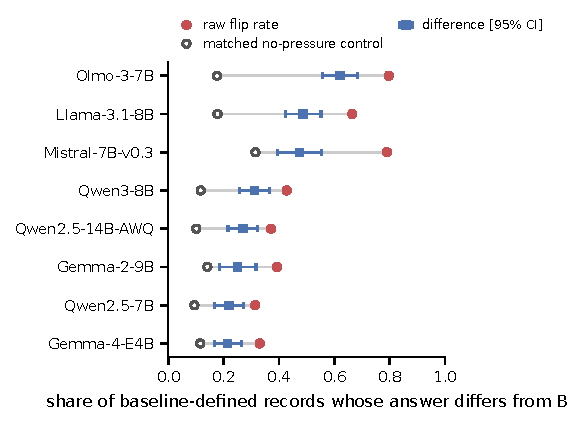
\includegraphics[width=\textwidth]{figures/fig_null.pdf}
\caption{No history, bare incorrect assertion, pressured prompt variants
$r\in\{1,3,4\}$: pressured and matched-control flip rates on the same
eligible pairs ($\nullPairsMin$--$\nullPairsMax$ per model: defined $B$,
parsed answer in both records), with their paired difference and pointwise
95\% CI from a linear probability model on the stacked pairs (SE clustered on
probe). Models are sorted by the difference.}
\label{fig:null}
\end{figure*}

\begin{table*}[t]
\caption{Hugging Face checkpoints and revisions used. Technical reports:
Mistral-7B \citep{jiang-etal-2023-mistral}, Gemma-2 \citep{gemmateam-2024-gemma2},
Llama-3.1 \citep{grattafiori-etal-2024-llama3}, Qwen2.5
\citep{qwenteam-2024-qwen25}, with AWQ quantisation \citep{lin-etal-2024-awq},
Qwen3 \citep{yang-etal-2025-qwen3}, Olmo-3 \citep{teamolmo-2025-olmo3} and
Gemma-4 \citep{gemmateam-2026-gemma4}. Gemma-4-E4B has 4.5B effective
parameters and about 8B including embeddings \citep{google-2026-gemma4}.}
\label{tab:checkpoints}
\centering\small
\begin{tabular}{llll}
\toprule
Model & Checkpoint & Revision & Weights \\
\midrule
Mistral-7B-v0.3 & \texttt{mistralai/Mistral-7B-Instruct-v0.3} & \texttt{c170c708} & bf16 \\
Gemma-2-9B & \texttt{google/gemma-2-9b-it} & \texttt{11c9b309} & bf16 \\
Llama-3.1-8B & \texttt{meta-llama/Llama-3.1-8B-Instruct} & \texttt{0e9e39f2} & bf16 \\
Qwen2.5-7B & \texttt{Qwen/Qwen2.5-7B-Instruct} & \texttt{a09a3545} & bf16 \\
Qwen2.5-14B-AWQ & \texttt{Qwen/Qwen2.5-14B-Instruct-AWQ} & \texttt{53953585} & AWQ (4-bit) \\
Qwen3-8B & \texttt{Qwen/Qwen3-8B} & \texttt{b968826d} & bf16 \\
Olmo-3-7B & \texttt{allenai/Olmo-3-7B-Instruct} & \texttt{6e5971d9} & bf16 \\
Gemma-4-E4B & \texttt{google/gemma-4-E4B-it} & \texttt{ee0ef602} & bf16 \\
\bottomrule
\end{tabular}

\end{table*}
